%Przykładowy plik ułatwiający złożenie projektu dyplomowego inżynierskiego.
%UWAGA: Generowany napis na stronie tytułowej o treści PROJEKT DYPLOMOWY INŻYNIERSKI został zaproponowany przeze mnie i nie jest, póki co, potwierdzony przez władze wydziału. Przed ostatecznym oddaniem tak złożonej pracy należy upewnić się jaka powinna być treść tego napisu. W momencie gdy uzyskam informację na temat treści tego napisu, dokonam niezbędnych zmian w źródłach.

\documentclass[eng,printmode]{mgr}
%opcje klasy dokumentu mgr.cls zostały opisane w dołączonej instrukcji

%poniżej deklaracje użycia pakietów, usunąć to co jest niepotrzebne
\usepackage{polski} %przydatne podczas składania dokumentów w j. polskim
\usepackage[utf8]{inputenc} %kodowanie znaków, zależne od systemu
\usepackage[T1]{fontenc} %poprawne składanie polskich czcionek
\usepackage{url}
%pakiety do grafiki
\usepackage{graphicx}
\usepackage{subfigure}
\usepackage{psfrag}
% \usepackage{color}
% \usepackage{xcolor}
%pakiety dodające dużo dodatkowych poleceń matematycznych
\usepackage{amsmath}
\usepackage{amsfonts}
\usepackage{supertabular}
\usepackage{array}
\usepackage{tabularx}
\usepackage{hhline}

\usepackage{color}
\usepackage{listings}		  %pozwalającyu listingować
\lstset{language=python, 
 		numbers=left,
 		showstringspaces=false,
 		numbersep=5pt,
 		basicstyle=\tiny}

%pakiet wypisujący na marginesie etykiety równań i rysunków zdefiniowanych przez \label{}, chcąc wygenerować finalną wersję dokumentu wystarczy usunąć poniższą linię
%\usepackage{showlabels}

%definicje własnych poleceń
\newcommand{\R}{I\!\!R} %symbol liczb rzeczywistych, działa tylko w trybie matematycznym
\newtheorem{theorem}{Twierdzenie}[section] %nowe otoczenie do składania twierdzeń
\renewcommand*{\lstlistlistingname}{Listingi}
%dane do złożenia strony tytułowej
\title{Narzędzie do detekcji i ekstrakcji zdarzeń akustycznych w materiale audio}
\engtitle{A tool for detecting and extracting acoustic events in an audio material}
\author{Konrad Kamil Janowski}
\supervisor{dr Maciej Walczyński, Katedra Akustyki i~Multimediów (W4/K5)}

%\guardian{dr hab. inż. Imię Nazwisko Prof. PWr, I-6} %nie używać jeśli opiekun jest tą samą osobą co prowadzący pracę

%\date{2008} %standardowo u dołu strony tytułowej umieszczany jest bieżący rok, to polecenie pozwala wstawić dowolny rok


\field{Elektronika (EKA)}
\specialisation{Inżynieria akustyczna (EIA)}

%tutaj zaczyna się właściwa treść dokumentu
\begin{document}
 
\bibliographystyle{apalike} %tylko gdy używamy BibTeXa, ustawia polski styl bibliografii
\maketitle %polecenie generujące stronę tytułową
\dedication{6cm}{Dla Rodziców, którzy zawsze mnie wspierali i~pozwolili mi rozwinąć się~w kierunku, w który pragnąłem.}

\small{\tableofcontents} %spis treści

\chapter{Wstęp}
\section{Cel i zakres pracy}
Przedmiotem pracy jest oprogramowanie do detekcji i~ekstrakcji zdarzeń akustycznych~w materiale audio. Oprogramowanie zostało stworzone do obsługi plików w formacie wave o rozdzielczości bitowej szesnaście(16) i dwadzieścia cztery(24) bity oraz częstotliwości próbkowania czterdzieści cztery i dziesięć setnych (44,1) kilo Herca i~czterdzieści osiem (48) kilo Herca. Oprogramowanie zostało przetestowane używając plików o~tych parametrach. Oprogramowanie zostało stworzone modularnie aby możliwy był jego dalszy rozwój. Z~powodu tego założenia, program ma możliwość obsługi dowolnej częstotliwości próbkowania oraz dowolnej rozdzielczości bitowej choć nie jest to zalecane. Praca w swojej logicznej strukturze zawiera cztery moduły:
\begin{enumerate}
\item Moduł odczytywania pliku,
\item Moduł przetwarzania sygnału,
\item Moduł detekcji zdarzeń,
\item Moduł zapisu wyników do pliku.
\end{enumerate}
Autor ma nadzieję, że zaprojektowany w~ten sposób system pozwoli na późniejszy rozwój i~ułatwi powtórne wykorzystywanie tego narzędzia.
\section{Motywacja}
Analiza nagrań odgrywa bardzo ważną rolę we współczesnych zastosowaniach akustyki. Jednym z~przykładów może być ochrona ludzi przed hałasem. Aby zbadać hałas na stanowisku pracy lub ocenić narażenie na hałas przestrzeni publicznej niejednokrotnie wykonuje się bardzo długie nagrania, trwające nawet kilkanaście godzin. Ze względu na metody analizy nieraz niezbędne jest wyselekcjonowanie z~nagrania konkretnych zdarzeń akustycznych i~analiza ich w izolacji, nie biorąc pod uwagę poziomu tła w pozostałym czasie. 

Z~drugiej strony, możemy wyobrazić sobie potrzebę wyizolowania z~nagrania bardzo wielu zdarzeń akustycznych, które wydarzają się w krótkim odstępie czasu. Jako przykład może tutaj posłużyć strzelnica, gdzie chcąc policzyć liczbę strzałów w ciągu dnia możemy zrobić nagranie krótkie i~na podstawie tego krótkiego wycinka czasu oszacować hałas podczas całego dnia. Innym razem możemy mieć potrzebę wykryć te zdarzenia do celów z~pozoru nie związanych z~akustyką. Gdyby ktoś chciał policzyć ile razy została odbita piłka do koszykówki podczas badania jej wytrzymałości, jednym z~możliwych sposobów na zliczenie liczby odbić mogłoby być policzenie zdarzeń akustycznych jakimi są odbicia piłki od ziemi. Być może ktoś ze względów medycznych chciałby sprawdzić, ile czasu w~ciągu jego snu zajmuje chrapanie i~w ten sposób ocenić jak duży problem ma z~tą dolegliwością. Również w~tym przypadku, przy pewnej kontroli hałasu środowiska mógłby zrobić to za pomocą stworzonego narzędzia. Jak widać, wyszukiwanie zdarzeń akustycznych wraz z~czasem ich trwania może być niezwykle użyteczne w wielu z~pozoru nie związanych z~tym dziedzinach. 

Biorąc pod uwagę, że przytoczone wyżej przykłady są jedynie wąskim wycinkiem zastosowań, które mogłyby przyjść do głowy komuś, kto ma wiedzę i~zainteresowanie w~innej dziedzinie niż autor pracy nie ulega wątpliwości, że warto posiadać takie oprogramowanie. Oczywiście wszystkie przytoczone sytuacje można analizować ręcznie, odsłuchując nagrane próbki. Analiza takich nagrań jednak pochłania dużo czasu i może być problematyczna. Z~pomocą stworzonego narzędzia można proces zupełnie lub częściowo zautomatyzować co w~obu przypadkach skutkuje znaczną oszczędnością czasu. 

Praca powstała w połowie z~chęci stworzenia użytecznego narzędzia a~w~połowie z~chęci autora do poznania współczesnych metod analizy cyfrowych sygnałów fonicznych. Rozwinięcie wiedzy w zakresie tworzenia oprogramowania w~języki Python, pracy z~systemem kontroli wersji oraz implementacja algorytmów znanych z~książek do realnie działającego programu jest procesem, który autor chciał zgłębić. Przedstawienie wyników w~formie zrozumiałej, czytelnej i~praktycznej jest nieraz jeszcze większym wyzwaniem i~nie można nabyć~w tym wprawy inaczej, niż pracując z~tymi wynikami i~samemu przekonać się na ile są one użyteczne.

Powyższe przesłanki zadecydowały o~stworzeniu narzędzia. 

\chapter{Wprowadzenie} \label{wprowadzenie}
W tym rozdziale zostaną wprowadzone podstawowe pojęcia, którymi autor posługiwał się podczas tworzenia pracy. Omówione zostaną teoretyczne podstawy problemu oraz ogólna struktura logiczna programu.
\section{Zdarzenie akustyczne}
Jak wspomniano w powyższym rozdziale, nie ma jednej ogólnej definicji zdarzenia akustycznego, które odnosi się do wszystkich dziedzin akustyki. Jedna z~możliwych definicji podana jest w~normie \cite{PN-ISO-1996-1:2006} dotyczącej akustyki środowiskowej. Zapis normatywny mówi:

\begin{quotation}
\textit{Należy podawać czas trwania zdarzenia~w odniesieniu do pewnej cechy dźwięku, jak np, liczba przekroczeń pewnego ustalonego poziomu. \newline \newline
Przykład: czas trwania zdarzenia można zdefiniować jako całkowity czas, w~którym poziom ciśnienia akustycznego mieści się w zakresie 10 dB maksymalnego poziomu ciśnienia akustycznego podczas zdarzenia\linebreak \cite{PN-ISO-1996-1:2006}.}
\end{quotation}

Biorąc pod uwagę przytoczone wcześniej możliwe zastosowania stworzonego oprogramowania powyższa definicja dobrze opisuje te sytuacje, które mają być detekowane. Ponadto, wykonanie oprogramowania, które rozpoznaje zdarzenia opisane w normie daje perspektywy na możliwości jego praktycznego zastosowania.
\section{Przyjęta definicja zdarzenia akustycznego}
W poprzedniej sekcji przytoczony został zapis normatywny, który opisuje zdarzenie akustyczne na potrzeby akustyki środowiskowej. Sugeruje on, żeby czas trwania zdarzenia akustycznego definiować jako całkowity czas, w~którym poziom ciśnienia akustycznego mieści się w~zakresie 10 dB maksymalnego poziomu ciśnienia akustycznego podczas zdarzenia. 
Nie można zapomnieć, że pomiary w~akustyce środowiskowej często wykonywane są przez długi czas. Dla przykładu, pomiar hałasu na stanowisku pracy może być wykonywany przez osiem godzin bez przerwy \cite{PN-ISO-9612:2011}. Plik z ośmiogodzinnych pomiarów może być monofoniczny, zapisany~w formacie wave~o częstotliwości próbkowania czterdziestu ośmiu kilo Herców(48 kHz) oraz rozdzielczości dwudziestu czterech bitów. Każda próbka takiego pliku zajmuje zatem dwadzieścia cztery bity w~pamięci a~każda sekunda zawiera czterdzieści osiem tysięcy próbek \cite{Principles_of_digital_audio}. Przy pomocy prostego wzoru możemy obliczyć jego rozmiar w pamięci komputera liczonej w bitach:
\begin{equation}
\text{rozdzielczość bitowa} * \text{częstotliwość próbkowania} * \text{długość pliku} = \text{rozmiar pliku}.
\end{equation}
\begin{equation}
24\;[b] * 48000\;[\frac{1}{s}] * 8*60*60\;[s] = 24\;[b] * 48000 \;[\frac{1}{s}] * 28800\;[s] = 3.31776*10^{10} \;[b] .
\end{equation}

Po przeliczeniu tego na jednostki bardziej sprzyjające interpretacji wyniku, przybliżając $1GB \approx 8*10^9\;[b]$, otrzymamy:


\begin{equation}
\frac{3.31776*10^10\;[b]}{8*10^9\;[\frac{b}{GB}]} = 4,1472\;[GB].
\end{equation}
Po dokonaniu takich obliczeń, można zauważyć, że przetwarzania takiego pliku nie jest zadaniem trywialnym. Jeżeli program wczytywałby cały plik do pamięci RAM, potrzebowałby on około czterech gigabajtów tej pamięci na samo obsłużenie pliku. Gdy dodamy do tego potrzebę pamięci operacyjnej dla samego programu, potrzeby systemu operacyjnego oraz innych aplikacji działających równolegle z~programem zauważamy problem w~postaci braku tych zasobów. Nowoczesne stacje robocze poradziłyby sobie z~takim obciążeniem, jednak należy pamiętać o~kilku rzeczach:
\begin{itemize}
\item Nie wszystkie firmy~i osoby fizyczne dysponują stacjami roboczymi, posiadającymi duże zasoby pamięci operacyjnej RAM,
\item plik może być dłuższy,
\item plik może zostać nagrany~z wyższą częstotliwością próbkowania,
\item może nastąpić potrzeba współdzielenia pamięci~z innymi programami bez możliwości ich wyłączenia.
\end{itemize}

Powyższe czynniki w głównej mierze skłoniły autora do tego aby swój program oprzeć o~przetwarzanie sygnału fragmentarycznie. Dokładny sposób działania programu zostanie omówiony w~dalszej części pracy. Co istotne w tym punkcie, wracając do definicji przytoczonej w normie \cite{PN-ISO-1996-1:2006}, zadaniem nietrywialnym jest osiągnąć jednocześnie obie te funkcjonalności:
\begin{enumerate}
\item Odczytywanie programu fragmentarycznie.
\item Zapamiętanie wszystkich poprzednich wartości próbek aby w razie potrzeby cofnąć się do poprzedniego fragmentu celem odnalezienia spadku poziomu~o 10 dB.
\end{enumerate}

Mając na uwadze powyższe przesłanki oraz możliwość późniejszego rozszerzania funkcjonalności programu, autor zadecydował się aby ograniczyć definicję zdarzenia akustycznego do definicji:

\begin{quote}
\textit{Należy podawać czas trwania zdarzenia~w odniesieniu do pewnej cechy dźwięku, jak np, liczba przekroczeń pewnego ustalonego poziomu. \linebreak \cite{PN-ISO-1996-1:2006}.}
\end{quote}

Powyższa definicja jest mniej praktyczna niż jej rozszerzona wersja. Wymaga ona wiedzy o~pewnych danych środowiska i~zdarzenia, jak np. poziom tła akustycznego oraz przewidywany poziom ciśnienia akustycznego generowany podczas zdarzenia. Pomimo świadomości tych ograniczeń autor postanowił zastosować tę uproszczoną definicję, aby program realizował fragmentaryczne przetwarzanie danych i~tym samym spełniał w~całości założenia pracy jednocześnie dając lepsze możliwości na jego rozwój w przyszłości. Autor ma nadzieję, że dodanie innego algorytmu do detekcji bazującego na przetwarzaniu sygnału partiami będzie prostsze niż przyszła zmiana samego centrum oprogramowania, czyli odczytywania i~zapisywania wyników. 

\section{Metoda wykrywania zakłóceń}

Na podstawie informacji,~o których mowa powyżej autor podjął decyzję aby wykrywać przekroczenia pewnego ustalonego poziomu ciśnienia akustycznego. Ciśnienie akustyczne to jednak określenie zbyt ubogie aby w pełni precyzyjnie opisać funkcjonalność narzędzia. Autor zdecydował się na zaczerpnięcie dodatkowych informacji z rozporządzeń normatywnych \newline\cite{PN-EN_61672-1:2014-03}. W związku z tym, program wykonuje następujące operacje:
\begin{enumerate}
\item Odnalezienie wszystkich plików wave i pliku referencyjnego w zadanym folderze,
\item odczytanie referencyjnego pliku wave o znanym poziomie dB SPL Z,
\item korekcja częstotliwościowa i~uśrednianie w~czasie zgodnie z~zaleceniami normy
  
\cite{PN-EN_61672-1:2014-03},
\item przeliczenie otrzymanych próbek na wartość dB FS,
\item odczytanie fragmentu pliku wave zawierające badany sygnał
\item korekcja częstotliwościowa i~uśrednianie w~czasie zgodnie z~zaleceniami normy 

\cite{PN-EN_61672-1:2014-03},
\item przeliczenie otrzymanych próbek na wartości dB FS,
\item przeliczenie otrzymanych wartości na wartości dB SPL poprzez porównanie ich~z wartością referencyjną,
\item wyszukanie przekroczeń ustalonego poziomu~i zapisanie do pamięci stanu programu(ilości znalezionych zdarzeń, zdarzeniu które miało początek na końcu przetwarzanego bloku),
\item repetycja punktów 4--8 aż do końca pliku,
\item segregacja odnalezionych zdarzeń,
\item ekstrakcja zdarzeń do osobnych plików wave w podfolderze folderu, w którym znajdowały się nagrania,
\item zapisanie wyniku do pliku w formacie .json,
\item repetycja kroków 4--12 dla wszystkich znalezionych plików wave,
\item wyświetlenie komunikatu o poprawnym zakończeniu działania programu.
\end{enumerate}
\section{Istniejące rozwiązania}
Autor nie spotkał się z rozwiązaniami programowymi, realizującymi podobną funkcjonalność. Niektóre mierniki poziomu dźwięku w podstawowym stopniu oferują tego typu rozwiązania, jednak autor nie znalazł informacji o żadnym, który umożliwia takie przetwarzanie na zapisanych uprzednio plikach.
\chapter{Metodologia} \label{metodologia}
W tej części zostanie omówiona metodologa przeprowadzonej pracy. Przedstawione zostaną narzędzia użyte to stworzenia programu, oprogramowanie, środowisko programistyczne oraz język programowania.
\section{System kontroli wersji - Git, GitHub, GitKraken}
\subsection{System kontroli wersji}
We współczesnym świecie istnieje bardzo wiele języków programowania. Każdy z nich~oferuje nieco inne możliwości i~funkcjonalności. Niezależnie jednak od wybranego języka, niezwykle istotnym jest system kontroli wersji. 

Jednym z~najpopularniejszych współcześnie systemów kontroli wersji jest Git. System kontroli wersji oferuje możliwość ciągłego śledzenia zmian w kodzie programu bez potrzeby ręcznego zapisywania wielu wersji pliku \cite{Git}. Problem wersjonowania oprogramowania jest znany od dawna i~jest jednym z~kluczowych zagadnień pracy nad programem, szczególnie kiedy pracuje się w~zespole. Gdy kilka osób pracuje nad jednym fragmentem kodu, wydaje się niemożliwe aby współpracować bez systemu kontroli wersji.

Pomimo iż praca dyplomowa inżynierska jest projektem jednoosobowym, system kontroli wersji spełnia swoją rolę i w~takim przypadku. Praca z~kodem jest nierozłącznie związana z~wielokrotnymi zmianami wcześniej wprowadzonych rozwiązań. Czasami wynika to z~faktu odkrycia nowych, lepszych rozwiązań. Bywają też przypadki, kiedy w zaawansowanym stadium pracy okaże się, że już na samym początku został popełniony błąd w~logice działania i~trzeba coś zmienić w~jedne funkcji. Często te zmiany wymagają powrotu do momentu pracy sprzed paru dni a~nawet tygodni, ponieważ kolejne fragmenty kodu opierały swoje funkcjonowanie na działaniu tych wadliwych elementów. Nie jest możliwym pamiętanie wszystkich tych zmian i~płynny powrót do nich poprzez przepisanie kodu. W takiej sytuacji, system kontroli wersji jest niezawodnym narzędziem, które pomaga zorganizować rozwój oprogramowania. 

Dodatkowo nie można nie docenić możliwości porównywania wersji roboczej pliku z~dowolną wersją tego pliku przechowywaną na serwerze. Daje to możliwość ocenienia wprowadzonych zmian, zastanowienia się czy wszystkie były konieczne oraz odpowiedniego przypomnienia sobie od czego zaczynaliśmy. Wszystkie te elementy pozwalają pracować w~sposób efektywny i~uporządkowany.

Ostatnim --- ale na pewno nie najmniej ważnym---elementem jest możliwość przechowywania całego programu na zdalnym serwerze. W~ dobie komputeryzacji bardzo często zdarza się, że pracujemy na kilku różnych urządzeniach nad tym samym projektem. Korzystając z~tego udogodnienia nie występuje problem przenoszenia danych pomiędzy urządzeniami. Dodatkowo w~razie utraty sprzętu postępy pracy nie zostają stracone.
 
Powyżej omówione aspekty jednoznacznie wskazują, że pracując nad oprogramowaniem, chcąc robić to w~sposób odpowiedzialny i~umożliwiający przyszłą współpracę korzystanie z systemu kontroli wersji jest nieodzownym elementem pracy. Dbanie o~czystość i~przejrzystość wprowadzanych zmian również jest elementem, którym powinna cechować się dobrze wykonana praca. 

\subsection{Git}
Jak zostało powiedziane, autor zdecydował się na skorzystanie z~Git'a jako systemu do kontroli wersji. Jest to bardzo popularny system. Oferuję prostotę obsługi, przejrzystość, dobrą możliwość współpracy w małych grupach. Dodatkowo twórcy Git'a oferują darmowe prywatne miejsca na serwerze do przechowywania danych. Dzięki temu gestowi oraz wymienionych wyżej zaletach autor zadecydował się wybrać właśnie ten system. 

\subsection{GitKraken}
Pomimo iż autor zadecydował się tworzyć oprogramowanie w ramach pracy dyplomowej inżynierskiej warto pamiętać o tym, że praca w przeznaczeniu jest skierowana do akustyków. W związku z tym poza efektywnością działania programu ważne jest też jego prostota i przejrzystość aby podczas pracy nad nim oraz przyszłej możliwej rozbudowy można skupiać się na istocie działania a nie odkrywaniu zawiłych sposobów obsługi oprogramowania towarzyszącego.

Git w wersji podstawowej jest dostarczany z~bardzo ubogim graficznym interfejsem użytkownika. Przykładowe okno zostało zaprezentowane na obrazie (\ref{git_gui})

\begin{figure}[hbtp]  
	\caption{Graficzny interfejs użytkownika GIT}
	\label{git_gui}   
	\centering
	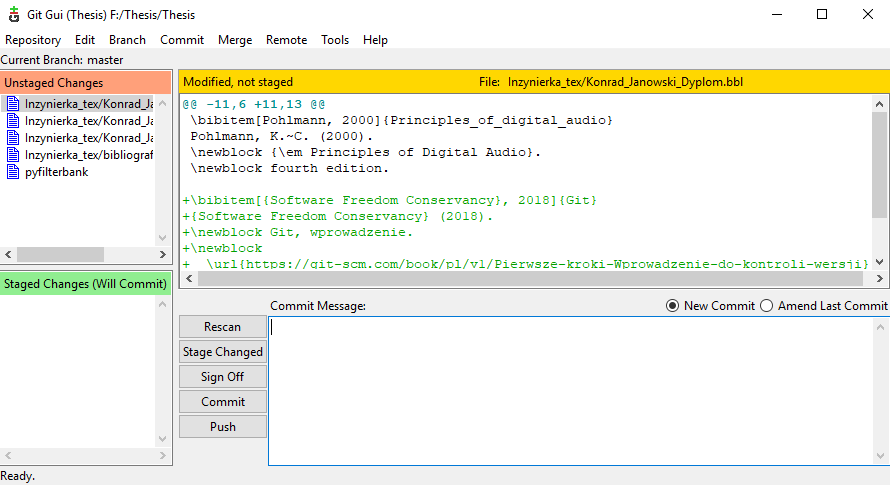
\includegraphics[width=0.8\textwidth]{git_gui.PNG}
\end{figure} 
 
Aby lepiej móc skupić się na logicznej strukturze programu autor zadecydował skorzystać z~programu GitKraken, który umożliwia pracę w~oparciu o system kontroli wersji Git w~bardziej przejrzystej i~czytelnej formie. Przykładowe drzewo kolejnych zmian zaprezentowano na obrazie (\ref{GitKraken})

\begin{figure}[hbtp]
\label{GitKraken}
\caption{Graficzny interfejs użytkownika programu GitKraken}
\centering
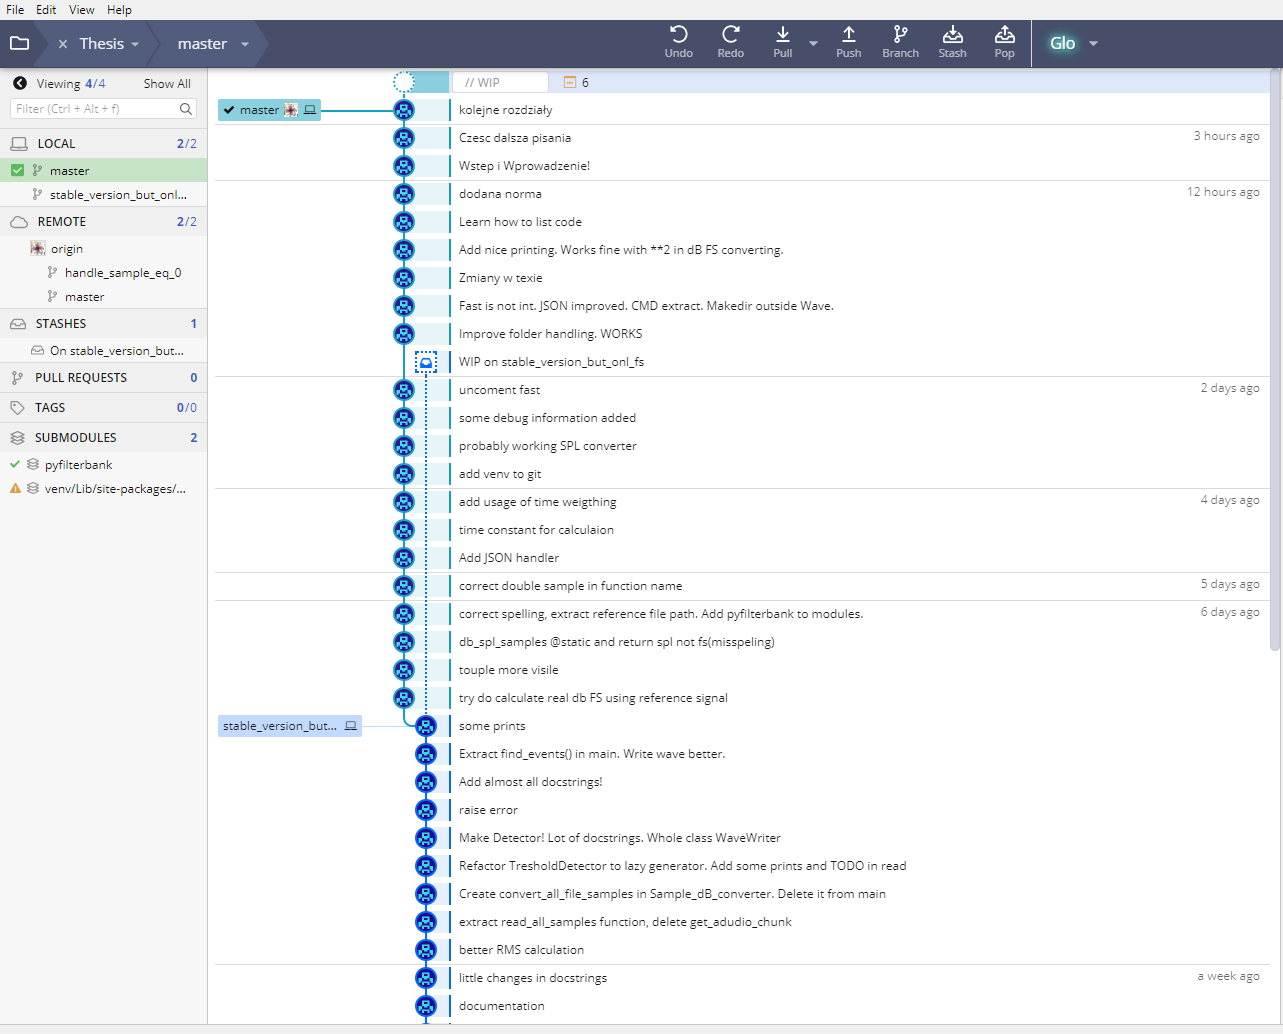
\includegraphics[width=0.8\textwidth]{GitKraken.PNG}
\end{figure}

W~opinii autora dobranie odpowiednich narzędzi jest bardzo istotne w~procesie tworzenia aplikacji. Wielu twórców oprogramowania, którzy nie są ukierunkowani na programowanie a~jedynie używają go jako narzędzia do wykonania innych czynności zaniedbuje wyżej wymienione aspekty dbałości o~czystość kodu. Dostęp i~odpowiednie użycie graficznych narzędzi, które są znacznie wygodniejsze i~bardziej intuicyjne niż ich konsolowe lub ubogie odpowiedniki z~pewnością może zachęcić twórców do większej dbałości o~ten aspekt tworzenia programów

\section{Język programowania - Python}\label{wybrany_jezyk}
Mając pomysł na działanie programu oraz niezbędne narzędzie do kontrolowania postępów prac należy wybrać język programowania, w~którym zostanie napisany program. Zdecydowano, że tym językiem będzie Python w wersji 3.7.1. Jest to najnowsza stabilna wersja tego języka \cite{Python_latest_release} w czasie tworzenia oprogramowania.

Wybrano Pythona z~kilku powodów. Python jest obecnie jednym z~najpopularniejszych języków programowania  \cite{Python_popular}. Rozwijanie programu i przyszła współpraca z~innymi twórcami może być dzięki temu ułatwiona. Łatwiej znaleźć innych ludzi posługujących się Pythonem niż innymi, mniej popularnymi językami. 

Dodatkowo Python jest prosty w składni, intuicyjny i ma nieduży próg wejścia. Nawet osoba, która nie jest doświadczona w~programowaniu może stworzyć podstawowe aplikacje. Oczywiście bardziej zaawansowane struktury wymagają wiedzy, umiejętności i~ doświadczenia ale ta początkowa intuicyjność daje szansę zapoznania się z nim niezawodowym programistom.

Ponadto Python ma rozbudowaną bazę bibliotek i~modułów, które można używać ponownie do swoich zastosowań\cite{Pypie}. Daje to ogromne możliwości tworzenia programów dopasowanych do potrzeb, korzystając z~gotowych modułów. Gdyby za każdym razem trzeba było zapisywać podstawowe operacje od nowa, proces kodowania byłby zdecydowanie dłuższy i~mógłby zajmować więcej czasu niż osoba zajmująca się inną dziedziną może przeznaczyć na opracowanie narzędzia. 

Do tego Python ma doskonale opracowaną dokumentację. Większość modułów jest opisana czytelnie i~zrozumiale. Zdecydowanie ułatwia to pracę z~tym językiem. 

Co ważne, Python jest językiem interpretowanym a nie kompilowanym  \linebreak\cite{Przewodnik_po_pythonie}. Oznacza to, że do działania potrzebuje interpretatora, który działa niezależnie od systemu operacyjnego i jego bibliotek. Co prawda spowalnia to nieco jego działanie w porównaniu to języków kompilowanych takich jak C++ ale daje lepszą możliwość dzielenia się oprogramowaniem. Można skonstruować interpreter tak, by mógł być wysłany razem z~kodem programu i osoba odbierająca bez problemu będzie mogła ten kod interpretować. W przypadku języków kompilowanych występują często problemu  z udostępnianiem kodu źródłowego właśnie ze względu na ich silna interakcję z systemem operacyjnym. W kontekście przyszłego rozwoju programu dla akustyków jest to ważny aspekt wyboru języka.

Z podanych powodów, Python został wybrany do napisania pracy.

Z wyborem Pythona wiąże się jeszcze jeden wybór, jego wersji. Obecnie najnowszą wersją jest Python 3.7.1 ale równocześnie wspierany jest Python w wersji 2.7.x \linebreak\cite{Python_latest_release}. Niestety, zmiana z~Pythona wersji drugiej na wersję trzecią wiąże się ze znaczącymi zmianami w~funkcjonalności języka i~wersje te nie są ze sobą kompatybilne. Wiele modułów aktualnie dostępnych do użytku dalej funkcjonuje w~wersji drugiej języka. Można by więc pokusić się o napisanie programu w starszej wersji. Python wersji drugiej przestaje jednak być wspierany wraz z końcem 2020 roku \cite{Python_end_of_life}. Oznacza to, że najprawdopodobniej ze względów bezpieczeństwa i~braku wsparcia większość nowych modułów będzie pisana w~Pythonie w~wersji trzeciej a~dodatkowo w~razie nieprawidłowości w działaniu wersji drugiej, nie będzie można liczyć na żadną pomoc.


\section{Środowisko programistyczne - Pycharm}
Pycharm jest środowiskiem dedykowanym do obsługi Pythona. Mając niewielkie doświadczenie z~tym środowiskiem autor wybrał je aby je poznać i~sprawdzić jego działanie. Każde środowisko oferuje odmienny zestaw funkcjonalności i~ułatwień użytkowania.

\section{Plik z informacjami o zdarzeniach: JSON}
Do reprezentacji wyników został wybrany format JSON opisany przez standard Ecma \linebreak\cite{JSON}. JSON, choć jego pełna nazwa brzmi "JavaScript Object Notation" jest uniwersalnym, popularnym sposobem wyświetlania i~przekazywania danych. O~jego wyborze przesądziła jego rosnąca popularność i~prostota użycia \cite{JSON_popular}. Dodatkowo, jest on łatwo odczytywany zarówno przez oprogramowanie jak i~przez człowieka co dodatkowo poprawia prostotę użytkowania. Do przekazania wyników i~ich obejrzenia nie potrzebujemy żadnego specjalnego oprogramowania, wystarczą standardowe aplikacje do odczytu plików tekstowych dostępne na większości systemów operacyjnych.
\chapter{Sposób działania oraz struktura programu} \label{struktura_dzialanie}
\section{Sposób działania programu - aplikacja konsolowa}\label{sposób}
Decydując się na program, należy wybrać w~jaki sposób będzie on uruchamiany. Może być jedynie biblioteką, czyli zestawem funkcjonalności, które mogą być wykorzystywane przez inny program. Jest również możliwość skonstruowania rozbudowanego graficznego interfejsu użytkownika. Na ten moment, autor zadecydował aby oprogramowanie działało jako program konsolowy. 

Oznacza to, że wywołuje się go z~konsoli systemu z odpowiednimi parametrami. Przykładowe wywołanie widzimy na obrazie(\ref{wywolanie}). Parametry wywołania i~struktura działania programu zostaną omówione w~dalszej części pracy.
\begin{figure}[hbtp]
\label{wywolanie}
\caption{Przykładowe wywołanie programu w konsoli systemu Windows}
\centering
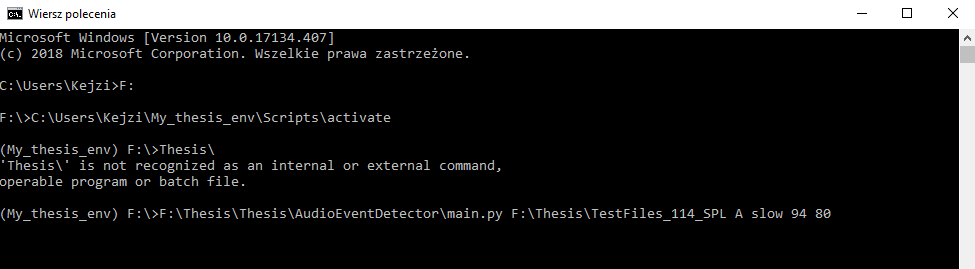
\includegraphics[width=0.8\textwidth]{cmd_wywolanie.PNG}
\end{figure}

Tego typu konstrukcja daje możliwość używania programu jako samodzielnego narzędzia. Jednocześnie, ze względu na ograniczony czas pracy nad programem stworzenie graficznego interfejsu mogłoby negatywnie wpłynąć na zadbanie o~poprawną funkcjonalność. W~ramach rozwoju programu autor nie wyklucza dodania graficznego interfejsu użytkownika do programu.

\section{Struktura programu}
Struktura plików w programie przedstawiona została na Rysunku (\ref{struktura}).

\begin{figure}[hbtp]
\label{struktura}
\caption{Struktura plików w programie}
\centering
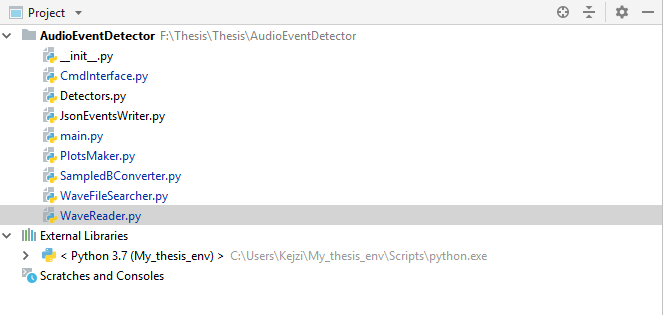
\includegraphics[width=0.8\textwidth]{struktura.PNG}
\end{figure}

Katalog "AudioEventDetector" zawiera wszystkie pliki źródłowe używane w programie. Na początku widzimy plik "\_\_init\_\_.py", który informuje interpreter Pythona, że 
katalog zawiera pythonowe pakiety \cite{init}. 

Plik "CmdInterface.py" odpowiada za komunikację z wierszem poleceń i odczytywaniem odpowiednich parametrów podanych przez użytkownika. "Detectors.py" to dwie klasy odpowiedzialne za detekowanie i~uporządkowanie zdarzeń akustycznych. "JsonEventWriter.py" zawiera funkcjonalność odpowiedzialną za zapisywanie wyniku to pliku .json. "main.py" to główna część programu, która wywołuje pozostałe moduły w~celu skonstruowania funkcjonalnej całości. "PlotsMaker.py" zawiera jedną klasę odpowiedzialną za zrobienie prostego wykresu z~danych. Nie jest ona używana w programie ale podczas rozwoju często przydaje się do wizualnej obserwacji danych. "SampleDbConverter.py" zawiera klasy odpowiedzialne za konwersję pliku z danych reprezentujących dynamiczny przebieg ciśnienia akustycznego na skorygowany częstotliwościowo uśredniony w czasie poziom ciśnienia akustycznego. "WaveFileSearcher.py" jest odpowiedzialny za odnalezienie plików wave do analizy oraz pliku referencyjnego."WaveRader.py" odpowiada za obsługę plików wave. Odczytuje fragmentami pliki na początku działania programu aby była możliwa ich analiza, na końcu programu zapisuje wybrane fragmenty do podfolderu. 

Uważny czytelnik zauważy, że wszystkie nazwy modułów zachowane są w jednej konwencji, nazwanej "CamelCase", co w~tłumaczeniu na polski można określić jako "StylWielbłąda". Autor zdecydował się na ten sposób notacji uwzględniając rekomendacje twórców języka \cite{PEP8}Używanie spójnego nazewnictwa jest o~tyle istotne, że pozwala się w~prosty sposób zorientować w strukturze programu. Jeżeli twórcy oprogramowania przestrzegają ustalonych, umownych zasad kod staje się z czasem coraz bardziej przejrzysty i~wymiana informacji jest dużo prostsza. 

\chapter{Szczegółowe omówienie funkcji w programie} \label{szczegolowe_omowienie}
W tym rozdziale na przykładzie kodu szczegółowo zostaną omówione główne funkcję programu. Dołożono wszelkich starań, żeby funkcje były omówione w kolejności jak najbardziej zbliżonej do logiki programu. Należy mieć jednak na uwadze, że niektóre funkcje wykorzystywane są kilkukrotnie co wyklucza zupełnie liniowe rozumienie kodu.

Warto w tym miejscu nadmienić, że istotnym elementem programu poza jego modularnością jako całości jest też zachowanie czystości kodu wewnątrz klas. Zasada pojedynczej odpowiedzialności, znaczących nazw jak i~inne dobre zasady pisania estetycznego kodu zostały zaczerpnięte z~literatury \cite{Czysty_kod}. Autor wierzy, że każdy kod powinien być możliwie łatwy do przeczytania przez człowieka, ponieważ to on jest głównym podmiotem pracującym nad nim. Być może zastosowanie tych zasad ułatwi a~może nawet i~uprzyjemni czytanie i~zrozumienie stworzonego kodu. 

Należy mieć na uwadze, że w~umieszczonych fragmentach kodu może się zdarzyć ominięcie niektórych wcięć. Spowodowane jest to szerokością kodu, który do odczytu w~środowiskach powinien mieć 150 \cite{PEP8}. Taka szerokość jednak nie pozwala na komfortowe umieszczenie listingu na stronie formatu A4. Dołożono wszelkich starań, aby wszystkie wcięcia istotne dla zrozumienia logiki kodu zostały zachowane
\section{Odnajdywanie plików wave}
Listing \ref{WaveFileSearcher} przedstawia metodę odnajdującą pliki wave w~zadanym folderze.

\begin{minipage}{\linewidth}
\begin{lstlisting}[caption={Fragment kodu źródłowego pliku WaveFileSearcher.py},captionpos=b,label={WaveFileSearcher}]
class WaveFileSearcher:
def find_wave_files_paths(self, ):
"""
Find wave files under path given in cmd. Path must be a directory containing wav files
and REFERENCE.wav file.
Returns
-------
   wave_files_and_reference_paths: [str]
        touple of two list. First is wave files paths to analize,
         second is reference file path.
"""
path = CmdInterface.get_path_from_cmd()
wave_files_paths = []
if os.path.isfile(path):
    raise NotADirectoryError('path is a file not a directory')
elif os.path.isdir(path):
    path_content = os.listdir(path)
    wave_files_paths = ["{}/{}".format(path, file_path) for file_path
    in path_content if (".wav" in file_path
                        or ".WAV" in file_path)and("REFERENCE" not in file_path)]
    reference_file_path = ["{}/{}".format(path, file_path) for file_path in path_content
                           if "REFERENCE" in file_path]
else:
    logging.error('{} is no valid path'.format(path))
    raise FileNotFoundError('{} is not a valid path'.format(path))

assert wave_files_paths, 'there is no any wave file under given path'
assert reference_file_path, 'there is no REFERENCE.wav file'
wave_files_names = [ntpath.basename(path) for path in wave_files_paths]

print('I found {} files. Files names are: {}'.format(len(wave_files_names), wave_files_names))
print('Found reference file under path: {}'.format(ntpath.abspath(reference_file_path[0])))
print('')

wave_files_and_reference_paths = (wave_files_paths, reference_file_path)
return wave_files_and_reference_paths

\end{lstlisting}
\end{minipage}
Pierwsze co zostało zapewnione w~tej metodzie to odporność na podanie niewłaściwej ścieżki do folderu. Program działa jedynie gdy zostanie podana ścieżka do folderu, który musi zawierać pliki wave oraz plik REFERENCE.wav. Jeżeli któregoś z tych elementów zabraknie, dostaniemy odpowiednie informacje o~błędach odpowiednio w liniach 13, 24 i~25. Dodatkowo widać w liniach 28--30 dodatkowe instrukcje print. Zostały wprowadzone w tym jak i~w innych modułach w celu informowania użytkownika o~tym, w~którym miejscu programu aktualnie się znajduje podczas pracy. Są to informacje pomocnicze, nie ostrzegające o błędach a~jedynie informujące o przebiegu. Pomagają jednak zorientować się, gdy przypadkiem ustawimy nie takie opcje jak byśmy chcieli. Główną funkcjonalność programu widzimy w liniach 14-19 w którym to tworzone są dwa obiekty, "wave\_files\_paths" oraz "reference\_file\_path". Są to listy, które zawierają odpowiednio ścieżki to plików wave, które zostaną poddane analizie oraz ścieżkę do pliku referencyjnego. Na koniec, w~linii 33. zostaje zwrócony obiekt zawierający obie te  wartości.

Dodatkowo można zauważyć tutaj kolejną konwencję nazewnictwa, klas, funkcji oraz zmiennych. Autor podczas całego programu stosował nazewnictwo zgodne ze standardem\linebreak\cite{PEP8}. Co ułatwia odnalezienie się w~programie.


\section{Odczytywanie pliku wave}
Na Listingu \ref{WaveFileReader}. został przedstawiony fragment kodu realizujący funkcję odczytywania odnalezionego pliku wave. 

\begin{minipage}{\linewidth}
\begin{lstlisting}[caption={Fragment kodu źródłowego pliku WaveFileReader.py},captionpos=b,label={WaveFileReader}]
def read_audio_data_chunk(self, seconds_to_read=30):
""" Read audio data in chunks.
Parameters
----------
    seconds_to_read: int
        define how many seconds will be read from file.
Returns
-------
    samples: [float]
        list of value of audio samples."""
chunk_size = seconds_to_read * self.frame_rate
total_length = round(self.audio_file.getnframes() / self.audio_file.getframerate(), 2)
print('Read file {}'.format(ntpath.abspath(self.file_path)))
print(('frame rate is {}, chunk size is {}'.format(self.frame_rate, chunk_size)))
print('total length is {} s'.format(total_length))

while True:
    start = self.audio_file.tell()

    print('Read samples from {} to {}'.format(start, start + chunk_size))
                                             
    samples = self.audio_file.readframes(chunk_size)

    print('Samples from {} to {} has been read'.format(start, self.audio_file.tell()))

    if not samples:
        print('End reading {}. Read {} frames '.format(ntpath.basename(self.file_path),
         self.audio_file.tell()))
        print('')
        self.audio_file.close()
        return
    print('')
    samples = self.decode_audio_chunk(samples)
    yield samples
\end{lstlisting}
\end{minipage}
Na Listingu \ref{WaveFileReader}. widzimy moduł odpowiedzialny za odczytywanie danych z pliku wave. Jak zostało wspomniane wcześniej, funkcja jest przystosowana to działania wielokrotnie i odczytywania pliku w kawałkach. Aby to umożliwić, funkcja została zaprojektowana aby była używana jako generator \cite{Generator}. Pozwala to na cykliczne zwracanie próbek, co dzieje się w linii 33. bez utraty informacji z poprzedniego wywołania. Istotnym elementem tej funkcji jest moment końca iteracji. Kiedy plik zostanie przeczytany do końca, zostaje wywołane słowo kluczowe "return"(linia 30) zamiast "yield"(linia 33). Jest to zgodne z rekomendacją do Pythona wersji trzeciej, \cite{return} która zmieniła działanie generatorów. W poprzednich wersjach przerwanie iteracji wykonywało się zazwyczaj poprzez instrukcję "raise(StopIteration)". 

Ilość czytanych danych jest z góry zdefiniowana w linii 1. Jest ona przeliczana w linii 11. na rozmiar czytanego fragmentu w bitach. 

\section{Konwersja pliku}
Konwersja pliku odbywa się wewnątrz piku SampledBConverter. 

Znajdują się tam dwie klasy:

\begin{minipage}{\linewidth}
\begin{lstlisting}[caption={Fragment kodu źródłowego pliku SampledBConverter.py,\newline klasa SamplesDbFSConverter},captionpos=b,label={SamplesDbFsConverter}]

class SamplesDbFsConverter:
"""Convert samples from given wave file to frequency and time weighted signal
 according to IEC 61672-1:2013"""

    def __init__(self, file_path):
        self.wave_reader_object = WaveReader(file_path)
        self.audio_samples_generator = self.wave_reader_object.read_audio_data_chunk()
        self.frequency_weighting = CmdInterface.get_frequency_weighting_from_cmd()
        self.time_weighting = CmdInterface.get_time_weighting_from_cmd()
        self.reference_db_spl_value = CmdInterface.get_reference_db_spl()
\end{lstlisting}
\end{minipage}

\begin{minipage}{\linewidth}
\begin{lstlisting}[caption={Fragment kodu źródłowego pliku SampledBConverter.py,\newline klasa SamplesDbSPLConverter},captionpos=b,label={SamplesDbSPLConverter}]

class SamplesDbSPLConverter(SamplesDbFsConverter):
    """Subclasses of SamplesDbFsConverter which add conversion to dB SPL"""
    def __init__(self, file_path, reference_db_fs_value):
        super().__init__(file_path)
        self.reference_db_fs_value = reference_db_fs_value

\end{lstlisting}
\end{minipage}

Zaprezentowano listing konstruktorów klas SamplesDbFsConverter (\ref{SamplesDbFsConverter}) oraz  SamplesDbSPLConverter (\ref{SamplesDbSPLConverter}). Jak widać, klasa SamplesDbSPLConverter dziedziczy po klasie SamplesDbFsConverter. Pokazuje to linia 2. Listingu \ref{SamplesDbSPLConverter}., gdzie widzimy odziedziczenie wszystkich metod i~w linii 5. wywołanie konstruktora klasy nadrzędnej. Rozwiązanie to zastosowano, ponieważ klasa SamplesDbFsConverter zostaje użyta to konwersji pliku referencyjnego. Gdyby od razu zaimplementować pełną funkcjonalności klasy SamplesDbSPLConverter, z oczywistej przyczyny referencyjna wartość "reference\_db\_fs\_value" nie mogłaby być jeszcze znana. 


Przyjrzyjmy się zatem bliżej metodom klasy SamplesDbFsConverter.

\begin{minipage}{\linewidth}
\begin{lstlisting}[caption={Fragment kodu źródłowego pliku SampledBConverter.py,\newline klasa SamplesDbFSConverter, metoda \_convert\_samples\_to\_db\_fs},captionpos=b,label={converttofs}]

    def _convert_samples_to_db_fs(self, energy_samples):
        """Convert samples in energy unit(preferably p^2) to dB FS according do AES17-2015.
        FS value is calculated from sample_width of read object.
        Parameters
        ----------
            energy_samples: [float]
                list of samples in energy unit (e.x p^2).
        Returns
        -------
            list(samples_db_fs): [float]
                list of samples in dB FS format.
        """
        max_value = 2**(self.wave_reader_object.sample_width*8-1)
        samples_db_fs = [10 * self._log_10_dealing_with_0((sample/max_value**2)*np.sqrt(2))
                         for sample in energy_samples]
        print('{} energy unit samples has been converted
        to {} samples dB FS'.format(len(energy_samples), len(samples_db_fs)))
        print('Full scale level is {}'.format(max_value))
        print('')
        return list(samples_db_fs)
    
\end{lstlisting}
\end{minipage}

Metoda \_convert\_samples\_to\_db\_fs pokazana na Listingu \ref{converttofs}. odpowiada za konwersję sampli do wartosci dB FS. W linii 14. na podstawie rozdzielczości bitowej zostaje obliczona maksymalna wartość cyfrowa, która mogła znaleźć się w odczytywanym pliku wave \cite{Cyfrowe_przetwarzanie_sygnalow}. Obliczenie wartości dB FS zostaje wykonane zgodnie z normą AES\linebreak \cite{AES17}. Ciekawym momentem jest linia 15., która wykorzystuje listę składaną do konstrukcji listy zawierającej przekonwertowane próbki. Listy składane pojawiały się już wcześnie w~programie. Do tej pory jednak działanie ich wynikało głównie z dbania o~czytelność kodu, listy składane bowiem często są bardziej zwięzłe i~czytelne niż ich klasyczne odpowiedniki \cite{Python_data_structures}. Tutaj jednak szczególnie istotne jest to, o~czym wspomniano w rozdziale \ref{wybrany_jezyk}. Język Python jest językiem interpretowanym, jednak część jego funkcji zostaje na poziomie interpretacji sprowadzona do kodu w języku C i~skompilowane, przez co działają z szybkością równą językom kompilowanym \cite{Wprowadzenie_python}. Jedną z~takich struktur jest lista składana. W widocznym przykładzie jest to o~tyle istotne, że wykonywanych jest wiele obliczeń i~czas ich wykonania jest istotnym elementem całego czasu działania programu.

\begin{minipage}{\linewidth}
\begin{lstlisting}[caption={Fragment kodu źródłowego pliku SampledBConverter.py,\newline klasa SamplesDbFSConverter,\newline metoda \_filter\_db\_samples\_with\_time\_constant},captionpos=b,label={filtertimeconstant}]
    def _filter_db_samples_with_time_constant(self, samples):
        """Take dynamic pressure samples and integrate it with time
        constant defined in IEC-61672-2013.
        Interact which command line do take time constant to use.
        Allowed constants are "slow" or "fast".

        Parameters
        ----------
            samples: [float]
                list of samples with dynamic pressure level.

        Returns
        --------
            time_weighted_samples: [float]
                list of samples weighted which defined time constant.

        """
        if self.time_weighting == 'slow':
            time_weighted_samples = standards.iec_61672_1_2013.slow(np.array(samples),
                                                            self.wave_reader_object.frame_rate)
            print("Slow constant is applied")
        elif self.time_weighting == 'fast':
            time_weighted_samples = standards.iec_61672_1_2013.fast(np.array(samples),
                                                            self.wave_reader_object.frame_rate)
            print("Fast constant is applied")
        else:
            raise ValueError('time weighting must be "slow" or "fast"
            , not {}'.format(self.time_weighting))

        print('{} samples has been converted to {} samples with {} time constant'.format(
        															len(samples),
                                                                    len(time_weighted_samples),
                                                                    self.time_weighting))
        print('')
        time_weighted_samples = list(time_weighted_samples)
        return time_weighted_samples
\end{lstlisting}
\end{minipage}

Na Listingu \ref{filtertimeconstant}. widzimy funkcję odpowiedzialną za uśrednienie sygnału w~czasie zgodnie z~normą  \cite{IEC-61672-2013}. Wartość stałej czasowej jest pobierana z~atrybutów klasy. W~tej metodzie zostały wykorzystane metody z biblioteki acoustics.standards \cite{acoustics}.

\begin{minipage}{\linewidth}
\begin{lstlisting}[caption={Fragment kodu źródłowego pliku SampledBConverter.py,\newline klasa SamplesDbFSConverter,\newline metoda \_filter\_samples\_with\_weighting\_filter},captionpos=b,label={filterweightingfilter}]
   def _filter_samples_with_weighting_filter(self, samples):
"""Filter samples with weighting filter. Use one of the weighting defined in IEC-61672.
 Weighting is defined in class variable.
        Parameters
        ----------
            samples: [float]
                list of samples representing dynamic pressure level.
        Returns
        -------
            weighted_samples: [float]
                list of samples representing weighted samples of dynamic pressure level.

        """

        weighted_samples = splweighting.weight_signal(samples,
                                                      self.wave_reader_object.frame_rate,
                                                      self.frequency_weighting)
        return weighted_samples
\end{lstlisting}
\end{minipage}


Listing \ref{filterweightingfilter} przedstawia metodę odpowiedzialną za filtrowanie próbek zgodnie z krzywą częstotliwościową A, B lub C zdefiniowane w normie \cite{IEC-61672-2013}. Wykorzystano tutaj funkcję weight\_signal() z biblioteki splweighting \cite{splweighting}.

\begin{minipage}{\linewidth}
\begin{lstlisting}[caption={Fragment kodu źródłowego pliku SampledBConverter.py,\newline klasa SamplesDbSPLConverter, metoda convert\_samples},captionpos=b,label={convertsamples}]
    def convert_samples(self,):
        """
        Make full conversion from dynamic representation to frequency and time
        weighted samples according to IEC-61672.
        Returns
        -------
            db_fs_samples: [float]
                frequency and time weighted full scale level.
        """
        while True:
            try:
                samples = next(self.audio_samples_generator)
            except StopIteration:
                return
            frequency_weighted_samples = self._filter_samples_with_weighting_filter(samples)
            time_weighted_samples = self._filter_db_samples_with_time_constant(
            frequency_weighted_samples ** 2)
            db_fs_samples = self._convert_samples_to_db_fs(time_weighted_samples)
            yield db_fs_samples
\end{lstlisting}
\end{minipage}


Listing \ref{convertsamples} pokazuje funkcję, która jest główną funkcjonalnością klasy. Wykorzystuje ona poprzednio omówione metody aby wykonać pełną konwersję pakietu danych. Widzimy więc w~liniach 11--14 obsługę generatora próbek. Linie 15--17 wywołują metody opisane poprzednio, aby w~linii 18. zwrócić pakiet próbek po korekcji czasowej i~częstotliwościowej. Wszystko opisane jest również jako generator, którego działanie kończy się gdy skończą się próbki, w~liniach 13--14. Nie jest tutaj wykonywana konwersja próbek na wartości dB SPL. Ta funkcjonalność zostaje rozszerzona w klasie SamplesDbSPLConverter.

\begin{minipage}{\linewidth}
\begin{lstlisting}[caption={Fragment kodu źródłowego pliku SampleSPLConverter.py,\newline klasa SamplesDbSPLConverter, metoda convert\_samples},captionpos=b,label={convertsamplesSPL}]
    def convert_samples(self,):
        """
        Make full conversion to dB SPL from dynamic representation to
        frequency and time weighted samples according
        to IEC-61672.
        Returns
        -------
            db_fs_samples: [float]
                frequency and time weighted full scale level.
        """
        while True:
            try:
                samples = next(self.audio_samples_generator)
            except StopIteration:
                return
            frequency_weighted_samples = self._filter_samples_with_weighting_filter(samples)
            time_weighted_samples = self._filter_db_samples_with_time_constant(
            frequency_weighted_samples ** 2)
            db_fs_samples = self._convert_samples_to_db_fs(time_weighted_samples)
            db_spl_samples = self.convert_samples_to_db_spl(list(db_fs_samples))
            yield db_spl_samples
 
\end{lstlisting}
\end{minipage}


Na Listingu \ref{convertsamplesSPL}. widzimy nadpisanie funkcji z~listingu \ref{convertsamples} rozszerzając ją o~linię 18., odpowiedzialną za konwersję na dB SPL. Aby prześledzić jej działanie należy spojrzeć na Listing \ref{samplesToDbSPL}.

\begin{minipage}{\linewidth}
\begin{lstlisting}[caption={Fragment kodu źródłowego pliku SampleSPLConverter.py,\newline klasa SamplesDbSPLConverter, metoda convert\_samples\_to\_db\_spl},captionpos=b,label={samplesToDbSPL}]     
      
def convert_samples_to_db_spl(self, db_fs_samples):
"""Convert samples in dB FS to dB SPL using reference value given in command line
Parameters
----------
    db_fs_samples: [float]
Returns
-------
    db_spl_samples [float]
    """
reference_db_spl_value = CmdInterface.get_reference_db_spl()
db_spl_samples = [reference_db_spl_value + (sample - self.reference_db_fs_value)
 for sample in db_fs_samples]
print('{0} dB FS {1} {2} samples has been converted to
{3} dB SPL {1} {2}samples'.format(len(db_fs_samples),
                                                                   self.frequency_weighting,
                                                                   self.time_weighting,
                                                                   len(db_spl_samples)))
print('Reference value was {0} dB FS {1} {2} '
      'with was equivalent to {3} dB SPL {1} {2}'.format(round(self.reference_db_fs_value, 2),
                                                         self.frequency_weighting,
                                                         self.time_weighting,
                                                         self. reference_db_spl_value, ))
print('')

return db_spl_samples




\end{lstlisting}
\end{minipage}

Za konwersję odpowiedzialna jest linia 11. Tam następuje porównanie obliczonej wartości dB FS z wartością referencyjną i~odpowiednia korekcja wskazania, zależna od zadeklarowanej wartości odniesienia w dB SPL oraz obliczonej wcześniej wartości odniesienia w~dB FS.
W ten sposób program konwertuje próbki z~reprezentacji dynamicznego ciśnienia akustycznego na skorygowany częstotliwościowo, uśredniony w czasie poziom ciśnienia akustycznego. W następnej części przyjrzymy się części odpowiedzialną za odnajdywanie i~organizowanie zdarzeń.
\section{Detekcja i organizacja zdarzeń}
Za detekcję i organizowanie zdarzeń odpowiedzialny jest plik "Detectors.py". Zawiera on dwie klasy, "count\_occurrence" oraz "organise\_events". Razem pozwalają na zdetekowanie i~przygotowanie w formie możliwej do dalszej analizy zdarzeń akustycznych. Moduł ten na razie zawiera tylko jedna klasę detekującą. W dalszym rozwoju możliwe jest dodanie kolejnych. Wystarczy aby każda z klas zwracała wyniki w~odpowiedniej formie a~wtedy dodając tylko jej wywołanie do struktury programu "main.py" będzie można dodać dodatkową detekcję zdarzeń. 

\begin{minipage}{\linewidth}
\begin{lstlisting}[caption={Fragment kodu źródłowego pliku Detectors.py,\newline klasa ThresholdCrossDetector, metoda count\_occurrence},captionpos=b,label={countoccurence}]     
    def count_occurrence(threshold, _last_previous_index=0, _found=0):
"""Detect starts and ends acoustic events. Events are all samples above threshold.
Parameters
----------
    threshold: float
        Variable which defined starts and ends events. Expected value depends on yielded data.
    _last_previous_index: int
        Internal variable use for keeping memory of previous data.
    _found: int
        Internal variable use for keeping memory of founded events.
Returns
-------
    events: [(float, float)]
        List of touples of two parameters. First defined detected value,
        second number of sampel in whole file
        If use properly it keep memory of previous data.
"""
while True:
    data = yield
    first_index_of_chunk = _last_previous_index
    _last_previous_index = len(data) + first_index_of_chunk
    events = []
    for value in data:
        if _found % 2 == 0 and value >= threshold:
            events += [(value, data.index(value)+first_index_of_chunk)]
            _found += 1
        if _found % 2 != 0 and value <= threshold:
            events += [(value, data.index(value)+first_index_of_chunk)]
            _found += 1
    yield events
\end{lstlisting}
\end{minipage}

Listing \ref{countoccurence} przedstawia funkcję znajdującą zdarzenia. Ponieważ cały program przetwarza plik we fragmentach, funkcja musi posiadać pamięć poprzednich zdarzeń i~zachować ciągłość zliczania odebranych próbek. Zapewniają to inicjalizacja wartości na liście inicjalizacyjnej w~linii  1. oraz następna ich aktualizacja z każdym przebiegiem funkcji. Lista inicjalizacyjna została użyta, aby z każdym wywołaniem generatora nie inicjalizować na nowo wartości, które są jedynie aktualizowane w liniach 19--20. Funkcja ta działa jako generator, pobierając dane w linii 18. oraz zwracając je w~linii 29. przy pomocy słowa kluczowego yield. Zliczanie zdarzeń odbywa się w~pętli w liniach 22--28.


\begin{minipage}{\linewidth}
\begin{lstlisting}[caption={Fragment kodu źródłowego pliku Detectors.py, klasa EventsOrganiser,\newline metoda organise\_events},captionpos=b,label={organiseevents}]  
    def organise_events(events, time_constant):
"""Search in events list and prepare easy to use list of touples.
Parameters
----------
    time_constant: str
        Time constant applied to a signal. Can be slow or fast.
    events: [(float, float)]
        List of two element touples.
        Must contain list of all events to organise where first value of every
        touple is value of sample, second is number of it position in file.
        Must contain every starts and endings of events(except first and last).
Returns
-------
    events_starts_ends_lengths: [(float, float, float)]
        List of three element touple which contains starts,
        endings and lengths of all founded events.
"""
time_constant_ms = {'slow': 1,
                    'fast': 0.125}
events_starts = [time*time_constant_ms[time_constant] for _, time in events[::2]]
events_ends = [time*time_constant_ms[time_constant] for _, time in events[1::2]]
events_length = []
events_starts_ends_lengths = []
for event_number in range(len(events_starts)):
    try:
        events_length.append(events_ends[event_number] - events_starts[event_number])
    except IndexError:
        print('there is an event which has only start')
        break
    events_starts_ends_lengths.append((events_starts[event_number],
                                       events_ends[event_number],
                                       events_length[event_number]))

if events_starts_ends_lengths:
    print('Events found are: {}'.format(events_starts_ends_lengths))
    print('')
return events_starts_ends_lengths
\end{lstlisting}
\end{minipage}

Kod pokazany na Listingu \ref{organiseevents}. odpowiada za zestawienie zdarzeń w formie umożliwiającą ich dalszą obróbkę. W liniach 18--20 zapisuje istotne cechy zdarzenia, biorąc pod uwagę stałą czasową  z~którą zostało dokonane przetwarzanie próbek. Linie 25--27 zabezpieczają działanie programu w przypadku gdy na nagraniu pojawi się zdarzenie, które nie kończy się w czasie nagrania. Ponieważ funkcja przyjmuje jako parametr wejściowy listę znalezionych zdarzeń nie musi być przygotowana do operowania na dużych ilościach danych. Przetwarzanie odbywa się więc jednorazowo dla wszystkich próbek. 
\section{Zapis pliku .json oraz plików wave}
Po przejściu poprzednich etapów, otrzymujemy gotowe dane ze zdarzeniami akustycznymi. Jedyne co pozostaje do zrobienia to zapisać je do pliku .json oraz wyekstrahować je z~pliku w~którym zostały znalezione. 

\subsection{JsonEventsWriter}
Przeanalizujmy działanie klasy JsonEventsWriter.

\begin{minipage}{\linewidth}
\begin{lstlisting}[caption={Fragment kodu źródłowego pliku JsonEventWriter.py,\newline klasa JsonEventsWriter},captionpos=b,label={jsonevents}] 
class JsonEventsWriter:
    def __init__(self, organised_events, file_name, destination_directory):
        self.organised_events = organised_events
        self.file_name = file_name
        self.destination_directory = destination_directory

    def create_events_in_json(self, ):
        events_for_json = {'All_Events': len(self.organised_events)}
        count = 1
        for event in self.organised_events:
            start, end, length = event
            events_for_json['Event_{}'.format(count)] = {'start': start, 
            						'end': end, 
            						'length': length}
            count += 1
        json_events = json.dumps(events_for_json)
        return json_events

    def save_json_to_file(self,):
        json_events = self.create_events_in_json()
        json_file_name = '{}_events.json'.format(self.file_name.replace('.wav',
         '').replace('.WAV', ''))
        json_file_path = '{}/{}'.format(self.destination_directory,
        								json_file_name)
        with open(json_file_path, 'w') as json_file:
            json_file.write(json_events)
        print('JSON file with events has been saved to: {}'.format(json_file_path))
        print('')
\end{lstlisting}
\end{minipage}

Klasa przedstawiona na Listingu \ref{jsonevents} posiada dwie metody, create\_events\_in\_json i~save\_json\_to\_file. Pierwsza z nich odpowiada za przygotowanie obiektu JSON w~Pythonie z~listy zawierającej zdarzenia akustyczne. Następnie korzystając z~tak przygotowanego pliku metoda save\_json\_to\_file zapisze je w pliku z rozszerzeniem .json, w~podkatalogu katalogu w~którym znajdowały się pliki audio.  Przykładowy plik zapisany przy pomocy tej klasy widzimy na listingu \ref{jsoncontent}. 

\begin{lstlisting}[caption={Przykładowa zawartość pliku .json},captionpos=b,label={jsoncontent}] 
{"All_Events": 2, "Event_1": {"start": 11, "end": 20, "length": 9},
 "Event_2": {"start": 30, "end": 43, "length": 13}}
\end{lstlisting}

\subsection{Ekstrakcja z plików wave}
Ostatnią czynnością jest ekstrakcja plików ze zdarzeniami akustycznymi z analizowanych plików. Zajmuje się tym klasa WaveWriter umieszczona w pliku WaveReader.py. Posiada ona dwie metody. Pierwszą z nich widzimy na listingu \ref{readdefinedframes}.


\begin{minipage}{\linewidth}
\begin{lstlisting}[caption={Fragment kodu źródłowego pliku WaveReader.py,\newline klasa WaveWriter, metoda read\_defined\_frames},captionpos=b,label={readdefinedframes}] 

   def read_defined_frames(self, file_path, event):
        """Read events from audio file
        Params
        ------
            file_path: str
                path to audio file which will be read
            event: (float, float, float)
                touple containing start, end and lenth of event
        Returns
        -------
            frames_and_params: (b, ())
                touple containing frames which event and params of file.
            """
        start, end, length = event
        audio_file = wave.open(file_path, 'rb')
        audio_file.rewind()
        frame_rate = audio_file.getframerate()
        start_position = audio_file.tell() + int(start * frame_rate)
        audio_file.setpos(start_position)
        frames_to_read = int(length * frame_rate)

        print('Read frames from {} to {}'.format(start_position, start_position + frames_to_read))

        frames = audio_file.readframes(frames_to_read)

        print('Samples from {} to {} has been read.'.format(start_position, audio_file.tell()))
        print('')

        params = audio_file.getparams()
        frames_and_params = (frames, params)
        return frames_and_params
\end{lstlisting}
\end{minipage}
Odczytuje ona tylko te bity plik wave, które zawierają znalezione zdarzenie akustyczne. Linie 15--21 odpowiadają za przygotowanie wskaźników na obsługiwanym pliku aby odczytać odpowiednią ilość bitów z odpowiedniego miejsca. Linia 25. odczytuje zadane wcześniej bity. Zwracana jest krotka zawierająca bity oraz parametry które powinny zostać nagrane do pliku wave. Metoda ta jest wywoływana przez drugą metodę, widoczną na Listingu \ref{writedefinedframes}.

\begin{minipage}{\linewidth}
\begin{lstlisting}[caption={Fragment kodu źródłowego pliku WaveReader.py,\newline klasa WaveWriter, metoda write\_defined\_frames },captionpos=b,label={writedefinedframes}] 
    def write_defined_frames(self, file_dir_path, frames_and_params, count):
        """Write frames to file under defined path.
        Params
        ------
            file_dir_path: str
                path to dir where file should be save.
            frames_and_params: (b, ())
                frames to write and params of audio file
            count: int
                value to different each event"""
        frames, params = frames_and_params
        file_name = '{}/event_{}.wav'.format(file_dir_path, count)
        audio_file = wave.open(file_name, 'wb')
        audio_file.setparams(params)
        audio_file.writeframes(frames)
        print('Wrote file {}'.format(file_name))
        audio_file.close()
\end{lstlisting}
\end{minipage}
Funkcja ta ma za zadanie zapisać odczytane wcześniej bity do pliku o nazwie stworzonej w linii 11. używając parametrów zgodnych z plikiem wejściowym. 
W ten sposób zamyka ona proces detekcji i ekstrakcji zdarzenia z zadanego pliku. 


\chapter{Użytkowanie programu} \label{uzytkowanie}
Ta część dotyczy sposobu użycia programu z punktu widzenia użytkownika.
\section{Sposób użycia}
Jak wspomniano w rozdziale \ref{sposób} program działa jako aplikacja konsolowa. Oznacza to, że wywołanie następuje poprzez wiersz poleceń systemu operacyjnego. Rozpatrzmy dokładniej wywołanie programu pokazane na Rysunku \ref{cmd}.

\begin{figure}[hbtp]
\caption{Przykładowe wywołanie z~wiersza poleceń}
\centering
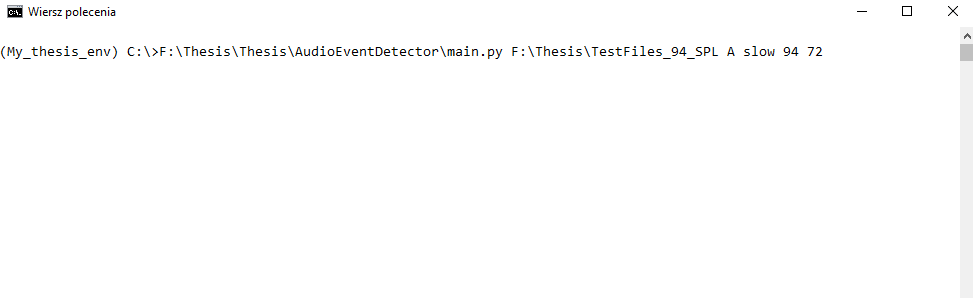
\includegraphics[width=0.8\textwidth]{cmd_wywolanie_2.PNG}
\label{cmd}
\end{figure}

Pierwsze co widzimy to napis (My\_thesis\_venv) przed samym wywołaniem. Oznacza to, że wiersz poleceń działa w wirtualnym środowisku Python \\ \cite{venv}. Nie jest to konieczne ale niezbędny jest interpreter Pythona w wersji 3.7.1. Następne jest 6 argumentów podanych do linii komend. Znaczenie każdego z~nich to:

\begin{minipage}{\linewidth}
\begin{enumerate}
\item To ścieżka prowadząca to pliku main.py, który uruchamia cały program,
\item To ścieżka do folderu, w którym znajdują się pliki wave oraz plik referencyjny,
\item Definiuje krzywą korekcji częstotliwościowej, która zostanie użyta do filtracji sygnału. Możliwe opcje to "A", "B" lub "C".
\item Definiuje stałą czasową, według której zostaną uśrednione próbki. Dopuszczalne wartości to "slow" oraz "fast".
\item To poziom w dB SPL pliku referencyjnego. Jeżeli sygnał referencyjny był o częstotliwości innej niż 1 kHz, lub użyty został mikrofon do którego wymagane jest wprowadzenie poprawki do odczytu z pistofonu poprawka ta musi zostać wprowadzona w tym miejscu. Dozwolona jest dowolna liczba zmiennoprzecinkowa mieszcząca się w zakresie typy float.
\item To próg wykrycia zdarzenia. Program odnajdzie wszystkie fragmenty pliku, który poziom mierzony w dB SPL przekroczy zadaną wartość. Dozwolona jest dowolna liczba zmiennoprzecinkowa mieszcząca się w zakresie typy float.
\end{enumerate}
\end{minipage}   

Należy zwrócić uwagę na strukturę folderu w którym trzymane są pliki do analizy. Przykładowa zawartość katalogu przedstawiona została na Rysunku \ref{katalog}

\begin{figure}[hbtp]
\caption{Przykładowa struktura katalogu z plikami wave}
\centering
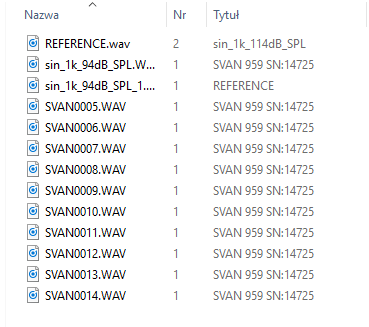
\includegraphics[width=0.8\textwidth]{katalog_przyklad.PNG}
\label{katalog}
\end{figure}

Na szczególną uwagę zasługuje plik REFERENCE.wav. Jest on niezbędny do zadziałania programu. Powinien znajdować się w nim sygnał referencyjny o znanym poziomie ciśnienia akustycznego. Nie może zawierać w sobie ciszy. Reszta plików może posiadać dowolne nazwy i być dowolnej długości. Jeżeli detekcja ma odbyć się prawidłowo niezbędne jest aby wszystkie pliki były nagrane tym samym zestawem pomiarowym bez zmian nastaw w czasie nagrań. Jeżeli wystąpi konieczność zmiany wzmocnienia podczas nagrania, należy nagrać nowy plik referencyjny i rozdzielić nagrania na dwa katalogi dzieląc je według parametrów nagrania. Po uruchomieniu programu możemy spodziewać się powstania katalogów ze znalezionymi zdarzeniami podobnych do tych pokazanych na Rysunku \ref{wydarzenia}.

\begin{figure}[hbtp]
\caption{Przykładowy katalog zawierający podkatalogi ze znalezionymi zdarzeniami}
\centering
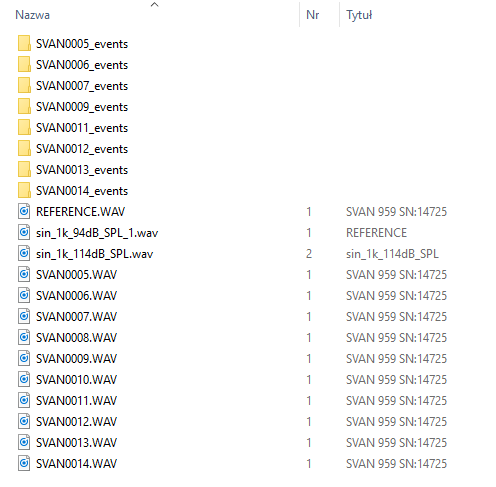
\includegraphics[width=0.8\textwidth]{katalog__eventy_przyklad.PNG}
\label{wydarzenia} 
\end{figure}

A zawartość każdego z nich powinna zawierać pliki .wav zawierające zdarzenia akustyczne oraz plik .json podsumowujący wyszukiwanie. Przykładowy wygląd podkatalogu prezentuje Rysunek \ref{podkatalog}.

\begin{figure}[hbtp]
\caption{Przykładowa struktura podkatalogu zawierającego zdarzenia }
\centering
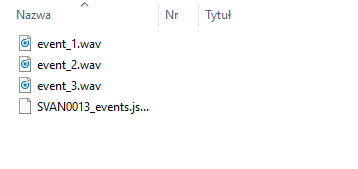
\includegraphics[width=0.8\textwidth]{podkatalog.PNG}
\label{podkatalog}
\end{figure}

\section{Zachowanie podczas normalnego działania}
Podczas normalnego działania program wypisuje do wiersza poleceń informacje o stanie jego działania. W razie błędu pomaga to zorientować się co go powoduje. Na Rysunku \ref{poprawne_dzialanie}. możemy zobaczyć przykład poprawnego działania programu a na Rysunku \ref{blad}. przykład wypisania informacji o błędzie spowodowanego nieprawidłowym wywołaniem programu. 

\begin{figure}[hbtp]
\caption{Przykład wiersza poleceń podczas poprawnego działania programu}
\centering
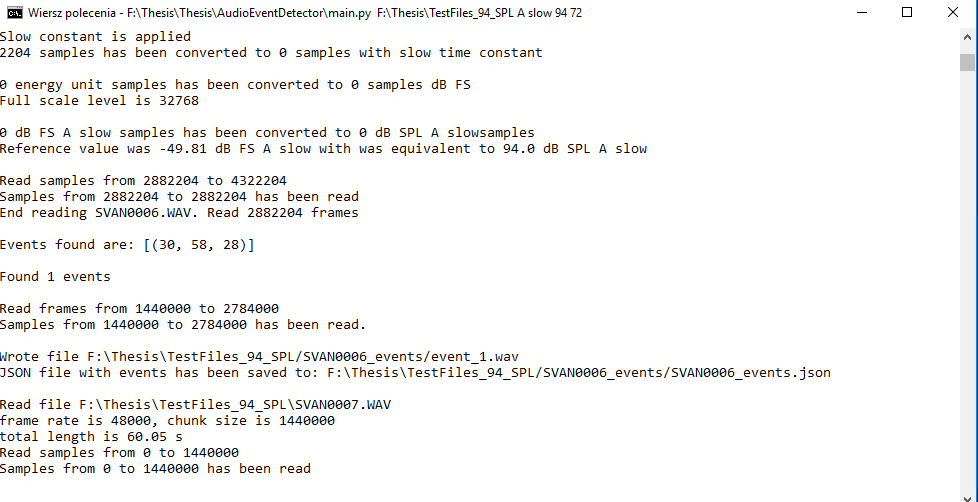
\includegraphics[width=0.8\textwidth]{poprawne_dzialanie.PNG}
\label{poprawne_dzialanie}
\end{figure}

\begin{figure}[hbtp]
\caption{Przykład wiersza poleceń podczas wykrycia błędu}
\centering
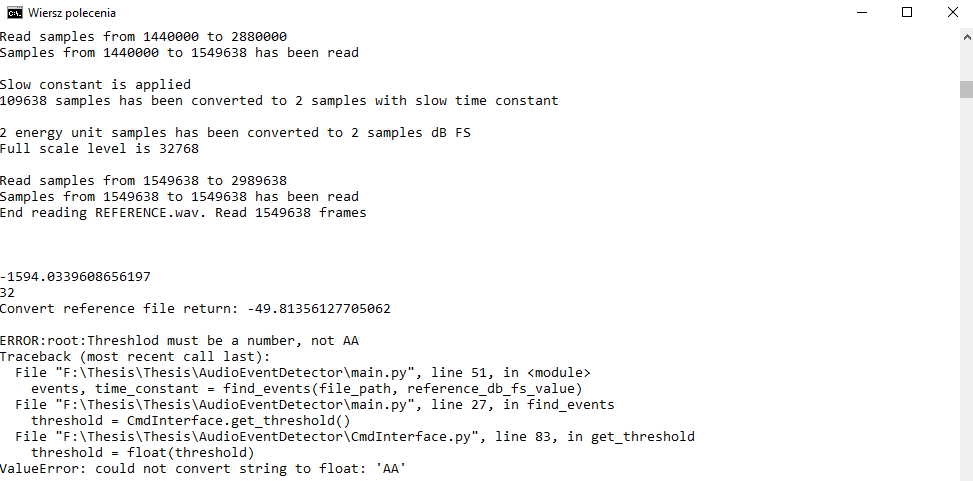
\includegraphics[width=0.8\textwidth]{blad.PNG}
\label{blad}
\end{figure}



\chapter{Testy} \label{testy}
W celu weryfikacji działania programu przeprowadzono testy. Próbki dźwiękowe nagrano przy pomocy miernika poziomu dźwięku Svantek 959 kalibrowanego kalibratorem Larson Davis CAL200. W celu kalibracji nagrano 3 pliki dźwiękowe, 2 z poziomem 94 dB SPL oraz jeden z poziomem 114dB SPL. Następnie nagrano różne zdarzenia akustyczne, następujące po sobie w zmieniającej się kolejności. Zdarzenia te to:
\begin{itemize}
\item szum różowy,
\item szum biały,
\item działanie odkurzacza,
\item działanie wiatraka,
\item uderzanie młotem w kowadło,
\item odtwarzanie muzyki z głośników laptopa,
\item wiatrak od komputera.
\end{itemize}

Nagrano łącznie 9 nagrań o różnej długości. Dodatkowo aby sprawdzić działanie programu podczas przetwarzania długich plików, za pomocą programu AudaCity stworzono jeden ponad pięciogodzinny plik składający się z kombinacji poprzednich, krótkich nagrań.

Poza czase pracy program nie wykazywał różnic w zachowaniu przy odczycie i zapisie plików krótkich jak i pliku długiego. Pomimo bardzo długiego plików zawierających wiele zdarzeń program nie obciążał urządzeń mocniej niż podczas normalnej pracy. Folder utworzony podczas pracy prezentuje Rysunek \ref{dlugiewyniki}.

\begin{figure}[hbtp]
\caption{Folder utworzony po przeszukaniu pliku o długości ponad 5 godzin}
\centering
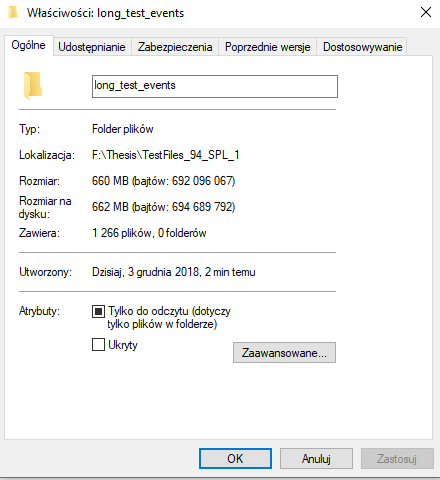
\includegraphics[width=0.8\textwidth]{long_file_found.PNG}
\label{dlugiewyniki}
\end{figure}

W celu weryfikacji czy program odnalazł tylko fragmenty zawierające zdarzenia akustyczne, posłużono się wizualizacją dostępną w programie AudaCity. Przykłady znalezionych zdarzeń prezentuje Rysunek \ref{znalezione_zdarzenia}. Zdarzenia zostały znalezione w pliku\linebreak "SVAN0007.wav" którego pełny przebieg wraz z~zaznaczonymi obszarami  gdzie zostały odnalezione zdarzenia oznaczono kolorem czerwonym pokazuje \ref{przebieg}. Podany przykład został przetestowany z~parametrami "A slow 94 85"

\begin{figure}[hbtp]
\caption{Zdarzenia akustyczne prezentowane w formie graficznej przy użyciu programu AudaCity}
\centering
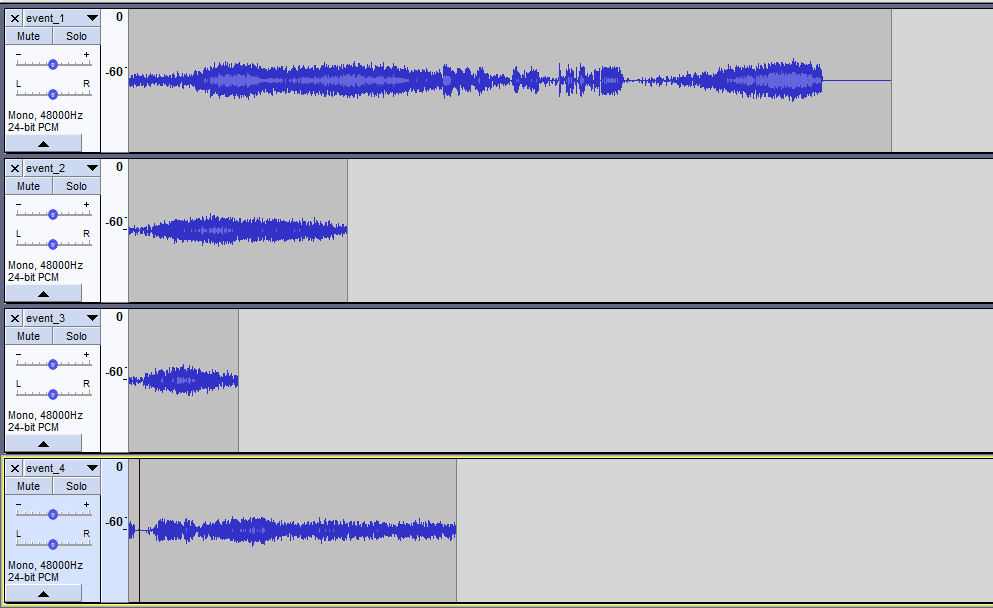
\includegraphics[width=0.8\textwidth]{zdarzeniaAuda.PNG}
\label{znalezione_zdarzenia}
\end{figure}

\begin{figure}[hbtp]
\caption{Wizualna reprezentacja pliku z którego ekstrahowano zdarzenia}
\centering
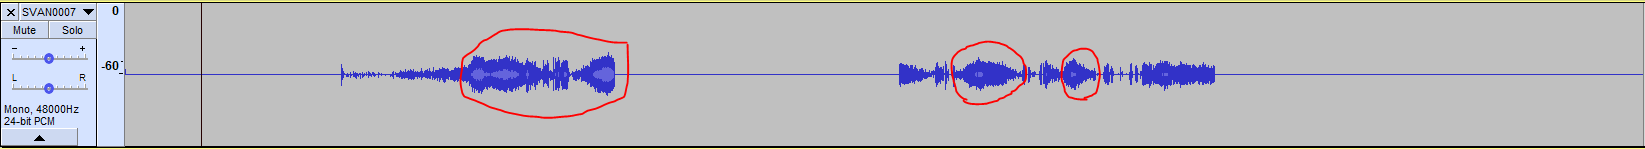
\includegraphics[angle=90,origin=c, scale = 0.6]{oryginalAuda.PNG}
\label{przebieg}
\end{figure}

Testy zostały przeprowadzone dla tych samych plików używają referencji z pliku 94 dB SPL oraz 114 dB SPL. W obu przypadkach program wyszukiwał tyle samo zdarzeń akustycznych we wszystkich plikach przy tym samym progu zadziałania. Testowano również stałe czasowe i różne krzywe ważenia. Dla wszystkich kombinacji program działał zgodnie z oczekiwaniami. 

\chapter{Podsumowanie}
Celem pracy było stworzenie oprogramowania, które umożliwia detekcję i~ekstrakcję zdarzeń akustycznych z~materiału audio. Na początku zadecydowano o~zawężeniu definicji zdarzenia akustycznego na potrzeby pracy. Zdarzenie akustyczne zdefiniowano jako przekroczenie pewnego poziomu ciśnienia akustycznego uśrednionego w~czasie zgodnie z~zadaną stałą czasową i~skorygowanego według zadanej krzywej korekcyjnej. Zagadnienie to zostało szerzej omówione w~rozdziale~\ref{wprowadzenie}. 

Następnym krokiem było dobranie odpowiednich narzędzi do pracy. W~rozdziale \ref{metodologia}. zostały przedstawione narzędzie użyte do stworzenia pracy. Zdecydowano się na korzystanie z~języka programowania Python w wersji 3.7.1, będącą najnowszą wersją języka podczas tworzenia oprogramowania. Dodatkowo autor zdecydował się na pracę z~systemem kontroli wersji Git przy pomocy oprogramowania GitKraken. Do pisania programu użyto środowiska programistycznego Pycharm. Aby w pełni zrealizować zamierzone cele, wykorzystano również standard zapisu danych JSON do przechowywania informacji o~odnalezionych zdarzeniach. 

W rozdziale \ref{struktura_dzialanie} przedstawiono sposób działania programu. Zdecydowano się na stworzenie aplikacji konsolowej. Omówiono również w podstawowym stopniu strukturę program.
 

Rozdział \ref{szczegolowe_omowienie} w~sposób szczegółowy omawia funkcjonalność programu. Przedstawione zostały listingi wybranych, najbardziej istotnych do zrozumienia logiki programu klas i~metod. Autor tłumaczy jak przebiega konwersja od nieskompresowanego sygnału wave, prezentującego dynamiczny przebieg ciśnienia akustycznego w~czasie na skorygowany częstotliwościowo uśredniony w czasie poziom ciśnienia akustycznego. Następnie objaśnia moduły odpowiedzialne za detekcję zdarzeń, ich organizację oraz sposób zapisu danych. 

Następnie rozdział \ref{uzytkowanie}. opisuje sposób użytkowania programu z punktu widzenia użytkownika. Zostają objaśnione parametry wejściowe oraz przygotowanie katalogów niezbędne do prawidłowego funkcjonowania. Zaprezentowany został również przykład zachowania programu podczas normalnego działania, zarówno poprawnego jak i~podczas wykrycia błędów użytkownika. 

Pracę zakończyły testy oprogramowania omówione w~rozdziale \ref{testy}. Program został użyty do detekcji zdarzeń w~plikach o~różnym czasie trwania, różnej zawartości oraz przy użyciu różnych plików referencyjnych. Oprogramowanie podczas przeprowadzonych testów zachowywało się w~sposób stabilny i~działało zgodnie z~oczekiwaniami. 

Efektem pracy jest oprogramowanie, działające jako aplikacja konsolowa. Może być użytkowane jako samodzielne narzędzie lub użyte jako element większego systemu. Oprogramowanie potrafi rozpoznać w~podanym pliku wave zdarzenia akustyczne, przekraczające zadany poziom dźwięku. Po detekcji następuje zapisanie wyników z ilością zdarzeń, oraz informacji gdzie się zaczynają, kończą oraz jaki jest ich czas trwania. Dodatkowo zdetekowane zdarzenia zostają zapisane jako pliki wave. Oprogramowanie przeszło podstawowe testy i działa zgodnie z~oczekiwaniami. Założenia pracy wspomniane na początku rozdziału zostały wobec tego spełnione.

Oprogramowanie poprzez swoją modularną budowę oraz dbałość autora o~czytelność kodu daje możliwości dalszego rozwoju. W przyszłości można rozbudować funkcjonalności programu o dodatkowe moduły, biorące pod uwagę bardziej szczegółowe cechu zdarzeń dźwiękowych. Najprostszym i~najbardziej pożądanym, zdaniem autora, usprawnieniem byłoby dodanie odnajdywania zdarzeń akustycznych na podstawie ich relatywnego poziomu względem tła, nie zaś bezwzględnego odgórnie ustalanego jak to ma miejsce w stworzonym oprogramowaniu. Dodatkowo można rozbudowywać je o moduły odnajdywania hałasów tonalnych, o~maksimach w wybranych pasmach częstotliwościowych, jedynie o~zadanym czasie trwania itd. Dodatkowym usprawnieniem mogłaby być również funkcjonalność odnajdywania wydarzeń nagrywanych w czasie rzeczywistym. Przetwarzanie zdarzeń małymi fragmentami daje dobre fundamenty do implementacji dodatkowych modułów działających w czasie rzeczywistym . Te i~inne usprawnienia z~pewnością mogą sprawić, że oprogramowanie ma szanse stać się narzędziem użytecznym w~praktyce inżynierskiej.
\appendix
\addcontentsline{toc}{chapter}{Bibliografia} %utworzenie w spisie treści pozycji Bibliografia
\bibliography{bibliografia} % wstawia bibliografię korzystając z pliku bibliografia.bib - dotyczy BibTeXa, jeżeli nie korzystamy z BibTeXa należy użyć otoczenia thebibliography
%opcjonalnie może się tu pojawić spis rysunków i tabel
\listoffigures
\lstlistoflistings
% \listoftables
\end{document}
